% ########################################################################################################################################
%
% This is the main latex file. Here we call for inputs from other files. We also define some of the main characteristics of the document.
%
% ########################################################################################################################################
%
% You likely only need to modify the "Main_Content__Write_your_essay_here.tex" file.
%
% ########################################################################################################################################

\documentclass[12pt,a4paper,oneside]{paper}
% Encoding and Language
\usepackage[utf8x]{inputenc}
\usepackage{csquotes}
\usepackage[main=english,portuguese]{babel}
\usepackage{iflang}
\usepackage{ragged2e}
\usepackage{makeidx}
\usepackage{multicol}
\usepackage[export]{adjustbox}
\usepackage{tikz-dependency}
\usepackage{fancyhdr}

% Font Configurations
\renewcommand{\rmdefault}{phv}
\renewcommand{\sfdefault}{phv}
\def\FontLn{% 16 pt normal
  \usefont{T1}{phv}{m}{n}\fontsize{16pt}{16pt}\selectfont}
\def\FontLb{% 16 pt bold
  \usefont{T1}{phv}{b}{n}\fontsize{16pt}{16pt}\selectfont}
\def\FontMn{% 14 pt normal
  \usefont{T1}{phv}{m}{n}\fontsize{14pt}{14pt}\selectfont}
\def\FontMb{% 14 pt bold
  \usefont{T1}{phv}{b}{n}\fontsize{14pt}{14pt}\selectfont}
\def\FontSn{% 12 pt normal
  \usefont{T1}{phv}{m}{n}\fontsize{12pt}{12pt}\selectfont}

% Font Encoding
\usepackage[T1]{fontenc}

% Page Geometry
\usepackage{geometry}	
\geometry{verbose,tmargin=2.cm,bmargin=2.cm,lmargin=2.cm,rmargin=2cm}

% Line Spacing
\usepackage{setspace}
\renewcommand{\baselinestretch}{1.25}

% Graphics and Figures
\usepackage{graphicx}
\usepackage{subfigure}
\usepackage{subfigmat}
\usepackage{float}

% Mathematics and Theorems
\usepackage{amsmath}
\usepackage{amsthm}
\usepackage{amsfonts}
\usepackage{dcolumn}
\usepackage{indentfirst}

% Comments and Verbatim
\usepackage{verbatim}

% Hyperlinks
\usepackage[pdftex]{hyperref}
\hypersetup{
    colorlinks,
    linkcolor=blue,
    anchorcolor=black,
    citecolor=cyan,
    filecolor=black,
    menucolor=black,
    urlcolor=teal,
    bookmarksopen=true,
    bookmarksnumbered=true
}

% Captions and References
\usepackage[figure,table]{hypcap}
\usepackage[format=plain]{caption}
\DeclareCaptionFont{georgia}{\small\fontseries{n}\fontfamily{georgia}\selectfont}
\captionsetup{labelfont=georgia,font=georgia}

% Bibliography
\usepackage[backend=biber,style=apa]{biblatex}

% Acronyms
\usepackage[printonlyused]{acronym}

% Lipsum (for placeholder text)
\usepackage{lipsum}

% Cleveref (for clever references)
\usepackage[\IfLanguageName{english}{english}{portuguese}]{cleveref}

% Colors
\usepackage{xcolor}
\usepackage{color}

% Custom Commands
\newcommand{\gray}[1]{\textcolor{gray}{#1}}

% Equation Numbering
\renewcommand{\theequation}{{\fontseries{n}\fontfamily{georgia}\selectfont\arabic{equation}}}

% Section and Subsection Fonts
\sectionfont{\Large\bfseries\fontfamily{lmss}\selectfont}
\subsectionfont{\large\bfseries\fontfamily{lmss}\selectfont}

\makeindex

\addbibresource{bibliography.bib}
\begin{document}
\pagestyle{fancy}
\fancyhf{} % Clear previous settings
\rhead{LIFE}
\lhead{Velocidade da Luz}

%TC:ignore
% #############################################################################
%
%                           ENTER YOUR NAME, ISTid, AND TITLE
% 
% #############################################################################



\def\title {}


% #############################################################################
%
%               DO NOT MODIFY THE LINES FROM HERE TO THE MAIN DOCUMENT BODY
% 
% #############################################################################

\thispagestyle {empty}
\begin{center}
\begin{minipage}[c][5cm][t]{\textwidth}
\begin{center}
\includegraphics[width=5cm]{../IST_A_RGB_POS.png}
\end{center}

\end{minipage}
\begin{minipage}[t][10cm][c]{\textwidth}
\centering
{\FontMb Laboratório de Introdução à Física Experimental} \\
\paragraph{}
\centering
{\FontLb\Huge \title{Experiência de Milikan}}
\paragraph{}
{\FontMb Estimativa da carga elétrica de gotículas de óleo eletrizadas em suspensão num fluido} \\
\paragraph{}
{\FontMb 2023}
\end{minipage}

\begin{minipage}[c][1.5cm][c]{\textwidth}
\centering
{\FontLn }
\end{minipage}

\begin{minipage}[c][1.5cm][c]{\textwidth}
\centering



\end{minipage}
\begin{minipage}[c][3cm][c]{\textwidth}
\centering
\renewcommand{\arraystretch}{1.4}

\maketitle

\vspace{-5mm}
\hline
\vspace{-3mm}
\begin{center}
\centering
\section*{\centering Objetivos}
    \vspace{-3mm}
\small
\justify
Pretende-se com este trabalho determinar a carga eléctrica de pequenas gotas de óleo, tendo como objetivo final mostrar que a carga eléctrica não aparece com uma quantidade qualquer mas sempre como um múltiplo de uma unidade fundamental: a carga do electrão. Deste modo, um corpo electrizado apresenta um excesso de carga de sinal positivo ou negativo, mas cuja valor é sempre um múltiplo do valor da carga elementar $q_{ele}= 1,602176634\cdot 10^{-19}\,$ C.
Traduz-se este facto dizendo-se que a carga eléctrica é \emph{quantizada}.

Dentro das várias experiências elaboradas para mostrar este facto, uma montagem clássica é a do físico americano Robert A. Millikan\footnote{Millikan recebeu o prémio Nobel da Física em 1923 pelos seus trabalhos sobre a determinação da carga do electrão e efeito fotoeléctrico.} (1869-1953), também chamada experiência da gota de óleo.
    
\end{center}
\hline


\end{minipage}
\begin{minipage}[c][2cm][c]{\textwidth}
\centering

\end{minipage}

\end{center} 
\normalsize
\cleardoublepage
\setcounter{page}{1}
\fontfamily{cmr}\selectfont
%TC:endignore
% #############################################################################
%
%                           BEGIN MAIN DOCUMENT BODY
%
% #############################################################################

\printindex

\section{\sf Conceitos fundamentais}
Em muitas das experiências descritas na literatura para determinacão da velocidade da luz foram utilizados feixes luminosos
pulsados (ou modulados), que percorrem determinados trajetos de maior ou menor comprimento (ver exemplo na Fig. \ref{fig:Fizeau}). 
No presente trabalho, utiliza-se como fonte luminosa um díodo (LED) que emite radiação  visível com um comprimento de onda (c.d.o.)
na zona do vermelho. A tensão de alimentação do díodo é sinusoidal de frequência $f_{\textrm{mod}}=50$ MHz, fazendo com que a
intensidade da luz emitida $I_{\textrm{diodo}}(t)$ seja \emph{modulada em amplitude} (AM, do inglês \emph{amplitude modulation}),
variando entre 0 e $I_0$ de acordo com a expressão

\begin{equation*}
	\label{eq:f_am}
		I_{\textrm{diodo}}(t) = \frac{1}{2}I_0 [1+ \sin ( 2\pi f_{\textrm{mod}} t)]
\end{equation*}
%A(t) \cdot \sin ( 2\pi \cdot f_{luz} \, t) = \underbrace{

\begin{figure}[H] 
    \centering 
	\includegraphics[width=0.35\textwidth]{./luz_images/Fizeau.JPG}
	\caption{Esquema do aparelho (Roda de Fizeau) para determinar a velocidade da luz utilizado por Fizeau em 1849.
    \label{fig:Fizeau}} 
\end{figure}

%\section{\sf Introdução}

\newpage
\subsection{\sf Base do método}
No presente trabalho, o feixe luminoso proveniente do LED emissor é forçado a percorrer um determinado trajeto de comprimento $L$, sendo em seguida a sua intensidade  detectada por um fotodíodo receptor (Fig. \ref{fig:Montagem}). Um par de espelhos colocados a 90$^\circ$ pode deslocar-se ao longo de uma calha, sendo assim possível variar o comprimento do trajeto. Os sinais de amplitude impostos ao emissor e captados no receptor são registados\footnote{Depois de uma deteção \emph{heteródina}, em que a frequência modulada é desviada de \\ 
$f_{\textrm{bat}}=$50.050 MHz -- 50 MHz  = 50 kHz. Esta operação permite a utilização de um osciloscópio simples de banda de frequências mais estreita.} 
nos canais de um osciloscópio funcionando em modo “XY” (sem base de tempo).

\begin{figure}[H] 
 \centering 
	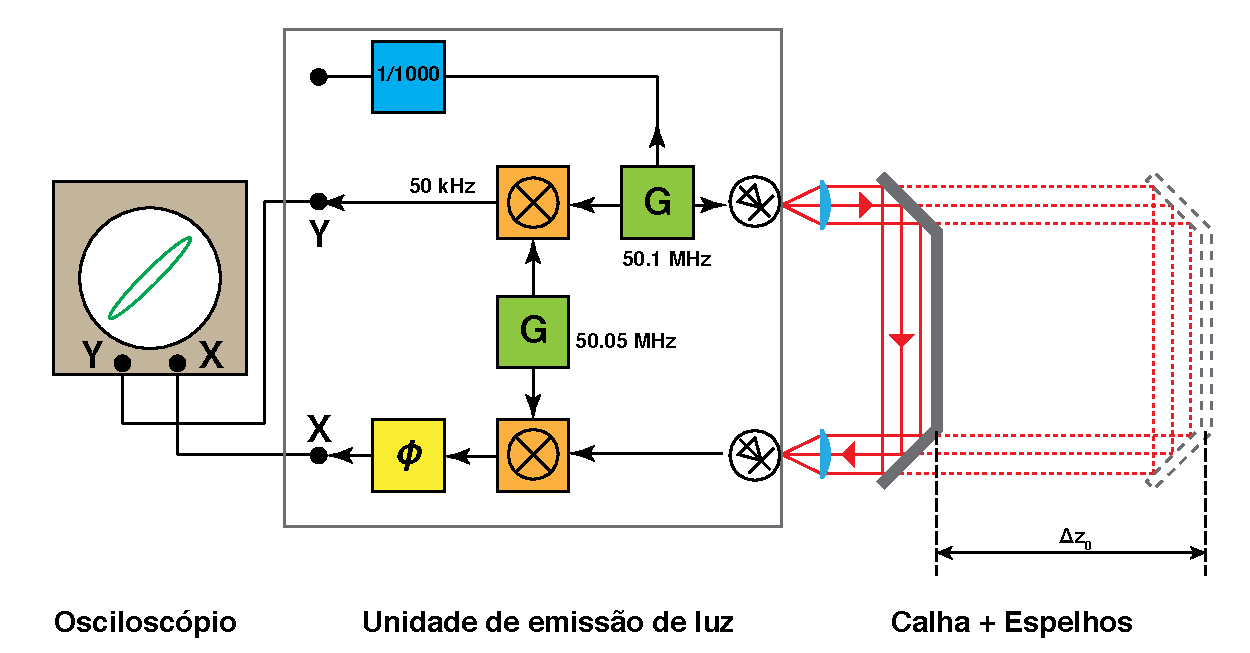
\includegraphics[width=01.0\textwidth]{./luz_images/esquema.pdf}
	\caption{Montagem para determinação da velocidade da luz. \label{fig:Montagem}} 
\end{figure}



Em ambos os canais X e Y (vertical e horizontal) a frequência é a mesma\footnote{Os sinais são \emph{coerentes}, pois provêm da
mesma fonte.}. No caso mais geral em que os sinais não estão em fase um com o outro, o padrão visualizado no osciloscópio é uma
\emph{figura de Lissajous}, neste caso uma elipse (Fig. \ref{fig:fase}), com um parâmetro $\delta$ dado pela equação geral:
\begin{equation}
	\label{eq:elipse}
	\sin^2 \delta = \frac{A_x^2}{A_{x0}^2} + \frac{A_y^2}{A_{y0}^2} - \frac{2 A_y\,A_x}{A_{y0}\,A_{x0}} \cos  \delta
\end{equation}
sendo $A_x(t)$ o sinal de intensidade captado no emissor,  $A_y(t)$ o sinal
proveniente do recetor, $A_{x0}$, $A_{y0}$ as respectivas amplitudes e $\delta$ a desfasagem entre os dois sinais. A desfasagem
relativa entre os sinais (e, logo, o ângulo $\delta$) varia com o comprimento do trajecto $L$ percorrido pelo raio luminoso.
Este efeito traduz-se numa variação da forma da elipse observada.  A elipse pode degenerar em retas quando os dois sinais estiverem
em fase, $\delta = 2n\pi$ (nos quadrantes ímpares)  ou em oposição de fase, $\delta = (2n+1)\,\pi$ (nos quadrantes pares). 

\begin{figure}[H] 
    \centering 
	\includegraphics[width=0.8\textwidth]{./luz_images/osci_fase.pdf}
	\caption{Figuras de Lissajous observadas no osciloscópio. À esquerda: sinais em fase; centro: sinais com uma dada desfasagem
    $\theta$; direita: sinais em oposição de fase.  \label{fig:fase}} 
\end{figure}

\subsection{\sf Velocidade da luz no ar}
Neste trabalho, a velocidade da luz é calculada a partir da determinação do comprimento do
caminho suplementar $\Delta L= 2\,\Delta z_0$ (ver Fig. \ref{fig:Montagem}) que a luz tem de percorrer para que se passe de
um extremo em que os sinais estão em fase ao extremo oposto de oposição de fase (ou vice-versa). Por definição, para passar de
uma situação à outra é necessário que o tempo gasto no percurso suplementar corresponda a metade de um período. Assim, a luz
percorre essa distância num intervalo de tempo $\Delta t$ igual a metade do período do sinal modulante, ou seja
$\Delta t=T/2=1/(2\cdot50\,\textrm{MHz})= 10\,\textrm{ns}$. 
No trajecto da luz no ar teremos a seguinte expressão para a sua velocidade:
\begin{equation}
	\label{eq:vc}
	c_{ar} = \frac{\Delta L}{\Delta t}=\frac{2\,\Delta z_0}{T/2} 
\end{equation}


\subsection{\sf Velocidade da luz em meios sólidos e líquidos}
 O índice de refração de um meio material $1$ em relação a outro meio $0$, para um dado comprimento de onda, é
 definido\footnote{Esta definição só é válida se as condutividades eléctricas dos meios $0$ e $1$ forem nulas, ou seja,
 nos \emph{dieléctricos} perfeitos.}
 como o quociente entre as velocidades de propagação da luz nos meios $0$ e $1$:

 \begin{equation}
	\label{eq:index}
	n_1 \equiv \frac{c_0}{c_1}  = \frac{\frac{1}{\sqrt{\varepsilon_0 \, \mu_0}} }{\frac{1}{\sqrt{\varepsilon_1 \, \mu_1}} } =
		\sqrt{\frac{\varepsilon_1 \, \mu_1}{\varepsilon_0 \, \mu_0}} = \sqrt{\varepsilon_r \, \mu_r}
\end{equation}

Nesta expressão $\varepsilon_0$, $\varepsilon_1$ ,	 $\mu_0$, $\mu_1$ são as constantes dieléctricas e as permeabilidades
magnéticas respetivamente do meios $0$ e $1$ e $\varepsilon_r$, $\mu_r$    as relativas $(\varepsilon_1= \varepsilon_r\, \varepsilon_0)$.

\begin{figure}[H]  
	\centering 
	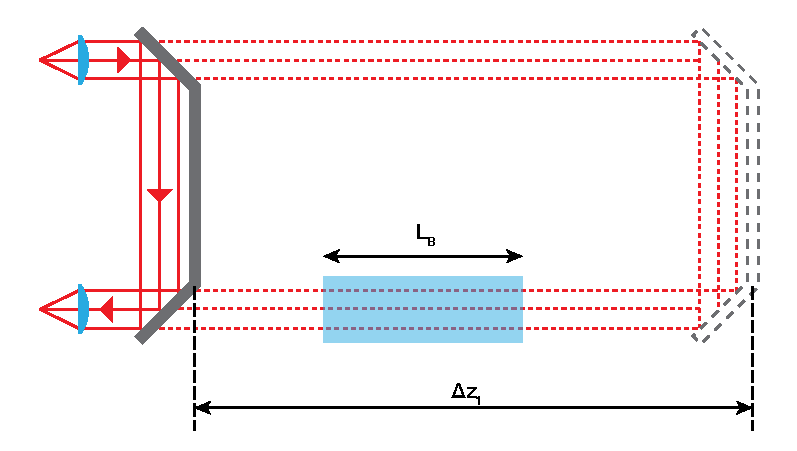
\includegraphics[width=0.8\textwidth]{./luz_images/esquema2.pdf}
	\caption{Montagem para determinar índices de refração em sólidos e líquidos. \label{fig:Montagem_bloco}} 
\end{figure}

Se no percurso do feixe luminoso interpusermos um bloco transparente de material sólido ou líquido de comprimento
$l_B$ (Fig. \ref{fig:Montagem_bloco}), o comprimento suplementar necessário $\Delta L$ entre as posições de fase e
oposição de fase vai variar. De facto, uma vez que as velocidades da luz nesse material e no ar são diferentes, a
desfasagem introduzida por uma dada espessura de material também difere da desfasagem causada pela mesma espessura de ar.
É pois necessário contabilizar em separado os tempos necessários para percorrer 
\begin{itemize}
\item o bloco de espessura $l_B$ à velocidade $c_B$
\item o restante comprimento $(2\Delta z_1-l_B)$ no ar à velocidade $c_{ar}$
\end{itemize}

Obtém-se assim a expressão

\begin{equation}
	\label{eq:vc_bloco}
	{T/2}  = \frac{2\,\Delta z_1 - l_B}{c_{ar}}  +  \frac{l_B}{c_{B}}
\end{equation}
em que $\Delta z_1$ é a nova posição em que se regista passagem de fase para oposição de fase (ou vice-versa). A partir
daqui calcula-se a velocidade $c_{B}$.  

Pode ainda obter-se o valor do índice de refração $n_{B}$ com a ajuda de (\ref{eq:vc}) e (\ref{eq:index}):

\begin{align}
	\label{eq:n_bloco}
	{T/2}  = \frac{2\,\Delta z_0}{c_{ar}}  &=  \frac{2\,\Delta z_1 }{c_{ar}} -   \frac{l_B}{c_{ar}}  +  \frac{l_B}{c_{B}} \nonumber \\ 
	\frac{2\,(\Delta z_0- \Delta z_1 )}{c_{ar}}  &= -   \frac{l_B}{c_{ar}}  +  \frac{l_B}{c_{B}} \nonumber \\
	\frac{2\,(\Delta z_0- \Delta z_1 )}{l_B} &= -1 +  \frac{c_{ar}}{c_{B}} \nonumber \\
	n_{B} &= 1 +  \frac{2\,(\Delta z_0- \Delta z_1 )}{l_B} 
\end{align}

Neste trabalho, serão  determinados os índices de refração e a velocidade da luz em  dois meios materiais: a resina
acrílica e a água. 
 


\newpage
\section{\sf Procedimento experimental}
\subsection{\sf Material}

    \begin{enumerate}
    \setlength{\itemsep}{0mm}
    \item Unidade de emissão (com amplitude modulada por um sinal de frequência 50 MHz) e de recepção de luz.
    % (díodos receptor) amplitude modulada por um sinal de frequência $50\,MHz$)(.
    \item Duas lentes plano-esféricas em suportes de tipo poste, ajustáveis
    \item Suporte móvel com dois espelhos planos para inversão do sentido de propagação da luz.
    \item Calha de aço inox.
    \item Banco óptico de altura ajustável.  
    \item Bloco de vidro acrílico transparente.
    \item Dois tubos com cerca de 1 metro de comprimento para conter água ou ar. 
    \item Osciloscópio de dois canais a funcionar em modo XY.
    \end{enumerate}

\subsection{\sf Trabalho preparatório} 
    \begin{enumerate}
    \item Preencha os objectivos do trabalho que irá realizar na sessão de laboratório. 
    \item Preencha o quadro com as equações necessárias para o cálculo das grandezas, bem como as suas incertezas. 
    \end{enumerate}


\subsection{\sf Regulação da montagem}
 
    \begin{figure}[H]  
        \centering 
        \includegraphics[width=0.5\textwidth]{./luz_images/fig5.jpg}
        \caption{Posicionamento das lentes no suporte da unidade de emissão de luz. \label{fig:lentes}} 
    \end{figure}

    \begin{enumerate}
    \setlength{\itemsep}{0mm}
    \item Comece por efectuar o alinhamento óptico do sistema. Ligue a unidade e posicione a lente junto ao LED emissor. Usando
    um alvo difusor (papel vegetal, por exemplo), observe a forma da mancha luminosa ao longo do percurso óptico, Ajuste a lente
    de modo a obter um diâmetro constante (feixe de raios paralelos, ou colimado) e à mesma altura relativamente à mesa. Note que
    pode ajustar a altura da lente, a sua posição transversal e a distância ao LED.
    \item Instale o conjunto de espelhos, assegurando-se de que o feixe incide em ambas as superfícies espelhadas (se for necessário,
    ajuste de novo a primeira lente, mas sem perder a forma do feixe que obteve). O suporte e os espelhos estão pré-alinhados, pelo
    que não deverá necessitar de ajustar os seus suportes. Verifique que os espelhos enviam o feixe de volta correctamente. Ainda sem
    a segunda lente, verifique que a mancha luminosa está centrada com  a janela do díodo receptor. Se não estiver, ajuste a primeira
    lente (e não os espelhos).
    \item Coloque agora a lente no lado do díodo receptor e, ajustando-a, alinhe o foco do feixe convergente de modo a incidir no
    centro do díodo (ver figura \ref{fig:lentes}).
    \item Ligue o osciloscópio às saídas da unidade emissora e visualize ambos os canais (modo DUAL). Optimize a posição da lente
    no díodo receptor de modo a maximizar a amplitude do \emph{sinal recebido}. Quando tiver terminado, volte a colocar o osciloscópio
    em mode XY e ajuste de modo a visualizar uma figura de Lissajous contida no écran.
    \item Coloque os espelhos na posição zero (posição $z_{\delta=0}$) da escala -- por exemplo, encostando o suporte dos espelhos
    ao suporte da unidade emissora. Rodando o botão da unidade que ajusta electronicamente a diferença de fase entre os dois sinais,
    obtenha uma reta dos quadrantes (ím)pares.
    \end{enumerate}
    \begin{figure}[H]  
        \centering 
        \includegraphics[width=0.6\textwidth]{./luz_images/fig6.jpg}
        \caption{Montagem para medição da velocidade da luz no ar. \label{fig:ar}} 
    \end{figure}

\subsection{\sf Medição da velocidade de propagação da luz no ar}
    \begin{enumerate}
    \item Desloque os espelhos sobre a calha e observe a modificação da figura no ecrã do 
    osciloscópio, em particular nas posições que correspondem a que os sinais recebidos estejam 
    em quadratura $(\delta=\pi/2)$ e oposição de fase $(\delta=\pi)$. Para esta última situação, registe a 
    nova posição $z_{\delta=\pi}$ dos espelhos e o intervalo de incerteza entre o qual os sinais parecem estar ainda em 
    oposição de fase (ver figura \ref{fig:ar}).
    \item Repita o procedimento para cada observador. 
    \item Calcule a velocidade de propagação da luz no ar $c_{ar}$, a sua incerteza e o desvio à exatidão\footnote{O valor $c_{ar}$
    é muito próximo de $c_{vacuo}$ = 299 792 458 m/s, que é uma constante exacta do Sistema Internacional de Medidas. O índice de
    refração do ar para a luz visível é $n_{ar}=1.000293$.}. 
    \end{enumerate}

    \begin{figure}[H]  
        \centering 
        \includegraphics[width=0.6\textwidth]{./luz_images/fig7.jpg}
        \caption{Montagem para medição da velocidade da luz no vidro acrílico. \label{fig:vidro}} 
    \end{figure}

\subsection{\sf Medição da velocidade de propagação da luz no vidro acrílico}
    \begin{enumerate}
    \item Verifique novamente se no zero da posição dos espelhos os sinais estão em fase. Usando o banco óptico, ajuste a altura
    e coloque cuidadosamente o bloco de vidro acrílico no percurso do feixe incidente, de modo a que incida perpendicularmente à
    face e usando o percurso mais longo no vidro acrílico (figura \ref{fig:vidro})
    \item Meça a posição $z_{\delta=\pi}$ e a incerteza correspondente dos espelhos para que os dois sinais detetados estejam em
    oposição em fase. 
    \item Repita a medição pelo menos duas vezes.
    \item Calcule o índice de refração obtido para o vidro acrílico, $n_{vidro}$, pela expressão (\ref{eq:n_bloco}), 
    e a sua incerteza. 
    \item Calcule o valor da velocidade da luz no vidro, $c_{vidro}$.

    \end{enumerate}

    \begin{figure}[H]  
        \centering 
        \includegraphics[width=0.6\textwidth]{./luz_images/fig8.jpg}
        \caption{Montagem para medição da velocidade da luz na água. \label{fig:agua}} 
    \end{figure}

\subsection{Medição da velocidade de propagação da luz na água}

    \begin{enumerate}
    \item Verifique a fase na posição inicial. Com o auxílio do banco óptico e dos dois suportes (ver figura \ref{fig:agua}),
    coloque cuidadosamente o tubo \emph{vazio} de modo a que o feixe incidente entre perpendicularmente à face. Pode desmontar
    este tubo para medir o comprimento interno do trajeto no ar/água.
    \item Registe a posição dos espelhos $z_{\delta=\pi}^{\textup{tubo}}$ que produz um sinal em oposição de fase. 
    \item Repita a medição para o tubo \emph{cheio de água} e obtenha o valor correspondente $z_{\delta=\pi}^{\textup{água}}$. 
    \item Calcule o valor do índice de refração $n_{\textup{água}}$ obtido, a sua incerteza e o desvio à
    exatidão\footnote{O valor tabelado é $n_{\textup{água}}=1.3330$.}. 
    \item Comente a precisão do valor da velocidade de propagação da luz obtida nos 
    diferentes meios.
    \end{enumerate}

\subsection{Análise, conclusões e comentários finais}
Discuta a qualidade dos dados obtidos e as conclusões que pode retirar desta experiência. Comente também sobre as condições
de realização da experiência, dos equipamentos utilizados e a influência de erros aleatórios e sistemáticos, identificando-os.\\

\HRule \\[0.5cm]


\newpage

\end{document}